\documentclass{beamer}
\usepackage{graphicx}
\usepackage{tikz}
\usetikzlibrary{shapes,arrows}
\usepackage{tikz}
%\usecolortheme{seahorse}
  \setbeamertemplate{footline}[page number]
\usepackage{multirow}
\setbeamertemplate{navigation symbols}{}
\setbeamertemplate{frametitle}[default][center]
\setbeamerfont{frametitle}{shape=\scshape}
\usepackage{color}

\usepackage{csquotes}

\usepackage{xcolor}

\usepackage[flushleft]{threeparttable}

{\title{\textsc{Econ 352 - Course Introduction} \\ \tiny (See Syllabus)}
\author{Trevor Gallen}
\date{}
\begin{document}
\renewcommand*{\inserttotalframenumber}{\pageref{lastframe}}


\setbeamertemplate{caption}{\raggedright\insertcaption\par}

\begin{frame}
\titlepage
\end{frame}

\begin{frame}
\frametitle[alignment=center]{Econ 352}
\begin{itemize}
\item Econ 352: Intermediate Macreconomics
\bigskip
\item Class:  T/Th, 7:30 a.m.-8:45 a.m. Rawls 3058
\bigskip
\item Me
\bigskip
\item Math:  MA 16010/16100/16500
\bigskip
\item My OH:  KRAN 315, Tuesdays 8:45-9:45
\bigskip
\item TAs:  Sayantan Roy (roy175@purdue.edu), Aaron Fehl (iguha@purdue.edu) 
\bigskip
\item TA OH:  Sayantan: Tuesdays, 1:30-2:30 p.m. in KRAN B024C
\item TA OH: Indulekha:   Mondays, 3:00-4:00 p.m. in KRAN 336B
\item My OH:   Tuesdays after Class, 8:45-9:45 a.m. in KRAN 315
\end{itemize}
\end{frame}

\begin{frame}
\frametitle[alignment=center]{Overview}
\linespread{1.6}
\begin{displayquote}
The purpose of this class is to give you a rigorous introduction to macroeconomic {\color<2->{red}{theory and empirics}}. We
examine longstanding stylized facts about both {\color<3->{red}{long-run growth}} and {\color<3->{red}{short-run fluctuations}} in macroeconomic aggregates through the focusing lens of theory. We study determinants of {\color<4->{red}{equilibrium}} in {\color<4->{red}{labor}}, {\color<4->{red}{consumption}},
{\color<4->{red}{investment}}, and money markets in particular. In doing so, we will also touch on money and banking and financial markets.
\end{displayquote}
\end{frame}

\begin{frame}
\frametitle[alignment=center]{Important Note}
\begin{itemize}
\item Today, we're going over the syllabus, and begin talking about the aggregates
\bigskip
\item It is incumbent on you to read it
\bigskip
\item All your accommodations should be given by {\color<2->{red}{September 5th}}.
\bigskip
\end{itemize}
\end{frame}

\begin{frame}
\frametitle[alignment=center]{Textbook}
\begin{figure}
\centering

\includegraphics[scale=0.3]{Williamson.png}
\end{figure}
\end{frame}

\begin{frame}
\frametitle[alignment=center]{Course Requirements}
\begin{itemize}
\item Two midterms ($2\cdot20\%=40\%$)
\bigskip
\item Seven minus one homeworks ($6\cdot3.\bar{3}\%=20\%$)
\bigskip
\item One final ($1\cdot30\%=30\%$)
\bigskip
\item I will give a bunch of little HotSeat questions.  Your total score on all questions will be worth 5\% of your grade.
\bigskip
\item The point totals all add up, so 1 point on the homework is the same as 1 point on a test (except HotSeat).  
\end{itemize}
\end{frame}

\begin{frame}
\frametitle[alignment=center]{Course Requirements}
\begin{figure}
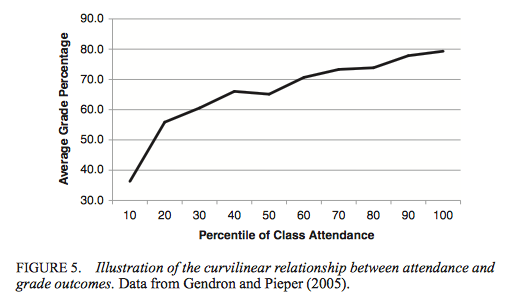
\includegraphics[scale=0.62]{Attendance.png}
\end{figure}
\end{frame}


\begin{frame}
\frametitle[alignment=center]{HotSeat}
\begin{itemize}
\item We'll use HotSeat a fair amount, including for next class
\bigskip
\item Please bring your cell phone .
\bigskip
\item If you do not have a cell phone, we can use a paper method
\end{itemize}
\end{frame}

\begin{frame}
\frametitle[alignment=center]{Participation}
\begin{itemize}
\item Participate in class (5\%!)
\bigskip
\begin{enumerate}
\item In person .
\bigskip
\item On discussion boards
\bigskip
\item Raise issue or suggest a fix on Github (https://github.com/trevorsgallen/Intermediate-Macroeconomics)
\end{enumerate}
\end{itemize}
\end{frame}



\begin{frame}
\frametitle[alignment=center]{Important Dates}
\begin{enumerate}
\item Aug 30th:  Homework 1 Due
\item Sep 13th:  Homework 2 Due
\item September 22nd:  Midterm I
\item Sep 27th:  Homework 3 Due
\item Oct 13th:  Homework 4 Due
\item October 27th:  Midterm II 
\item Nov 1st:  Homework 5 Due
\item Nov 15th:  Homework 6 Due
\item Dec 6th:  Homework 7 Due
\item TBD soon:  Final Exam
\end{enumerate}
\end{frame}

\begin{frame}
\frametitle[alignment=center]{Cheating}
\begin{itemize}
\item Becker 1968, Crime and Punishment: An Economic Approach
\begin{displayquote}
There was a tendency during the eighteenth and nineteenth centuries in Anglo-Saxon countries (and even today in many Communist and underdeveloped countries) to punish those convicted of criminal offenses rather severely, at the same time that the probability of capture and conviction was set at rather low values.  [...]  a reduction in [the probability of being caught] obviously reduces expenditures on combating crime, and, since the expected punishment is unchanged, there is no ``obvious" offsetting increase in [crime.  Therefore, a society might] keep police and other expenditures relatively low and to compensate by meting out strong punishments to those convicted.
\end{displayquote}
\item Don't cheat.  
\end{itemize}
\end{frame}

\begin{frame}
\frametitle[alignment=center]{Expected Grade Distribution}
\begin{itemize}
\item Broad expectation: real results may vary.
\bigskip
\item All grades, naively summed, then curved, roughly minimize the within-category variance/maximize between-category variance:
\begin{table}
\begin{tabular}{lccc}
A+ & 3.22\% & \\
A & 14.82\% & 29.73\%\\
A- & 11.70\% & \\
B+ & 11.26\% & \\
B & 20.71\% & 41.59\%\\
B- & 9.62\% & \\
C+ & 6.86\% & \\
C & 11.35\% & 21.74\%\\
C- & 3.52\% & \\
D+ & 1.17\% & \\
D & 1.98\% & 3.66\%\\
D- & 0.51\% & \\
F & 1.85\% & 1.85\%\\
\end{tabular}
\end{table}
\end{itemize}
\end{frame}

\begin{frame}
\frametitle[alignment=center]{Emergencies}
\begin{itemize}
\item This syllabus is subject to revision in the event of a major campus emergency or other circumstances beyond the instructor's control.  For instance, we may have to change weighting, or the time of the final exam.
\bigskip
\item See ``Emergency Preparedness Document" and links for details on emergency preparedness \& notification
\end{itemize}
\end{frame}

\begin{frame}
\frametitle[alignment=center]{Questions}
\begin{itemize}
\item Any questions?
\end{itemize}
\end{frame}


\end{document}